\RequirePackage{amsthm} %https://tex.stackexchange.com/questions/687324/unknown-theoremstyle-warning-with-springer-nature-template
\documentclass[sn-mathphys-num,iicol]{sn-jnl}

%\usepackage{sn-jnl.sty}
\usepackage{graphicx}%
\usepackage{multirow}%
\usepackage{amsmath,amssymb,amsfonts}%
\usepackage{amsthm}%
\usepackage{physics}
\usepackage{siunitx}
\usepackage{mathrsfs}%
\usepackage[title]{appendix}%
\usepackage{xcolor}%
\usepackage{textcomp}%
\usepackage{manyfoot}%
\usepackage{booktabs}%
\usepackage{algorithm}%
\usepackage{algorithmicx}%
\usepackage{algpseudocode}%
\usepackage{listings}%
\usepackage{newtxmath}%
\usepackage[tiny]{titlesec}%
\usepackage[ngerman]{babel}
\usepackage{booktabs}

\theoremstyle{thmstyleone}
\newtheorem{theorem}{Theorem}
\newtheorem{proposition}[theorem]{Proposition}

\theoremstyle{thmstyletwo}
\newtheorem{remark}{Remark}

\theoremstyle{thmstylethree}
\newtheorem{definition}{Definition}

\raggedbottom

\newcommand{\td}{\text{d}}

\titleformat{\subsection}{}{\thesubsection}{1em}{\itshape}
\titleformat{\subsubsection}{}{\thesubsubsection}{1em}{\itshape}

\begin{document}

\title[]{Praktikum 4 -- Versuch 425: Elektronisches Rauschen}
\author*[1]{\fnm{Jonas} \sur{Wortmann}}\email{s02jwort@uni-bonn.de}
\author*[1]{\fnm{Angelo} \sur{Brade}}\email{s72abrad@uni-bonn.de}
\affil*[1]{Rheinische Friedrich--Wilhelms--Universität, Bonn}

\maketitle

\section{Einleitung}
In jedem elektrischen Schaltkreis ist ein elektronisches Rauschen vorhanden.
Dieses Rauschen setzt sich z.B. aus dem \textsc{Johnson}--Rauschen und dem Schrotrauschen zusammen, wobei auch Randbeiträge, wie dem Rauschen von Verstärkern, berüchsichtigt werden.
Das \textsc{Johnson}--Rauschen ist temperaturabhängig, daraus lässt sich die \textsc{Boltzmann}--Konstante bestimmen.
Das Schrotrauschen wird durch die Quantelung der Elementarladung hervorgerufen.
Die Größe der Elementarladung lässt sich damit bestimmen.

\section{Bandbreite}
\subsection{Theoretischer Hintergrund}
\footnote{Die relative Abweichung des Fehlers vom Messwert und die Abweichung vom Literaturwert in $\sigma $ wird immer hinter dem Messwert wie $[\cdot \%,\cdot \sigma ]$ angegeben.}Die Bandbreite gibt die Breite eines Frequenzsbands an.
Da das elektronische Rauschen von der Bandbreite abhängig ist, wird diese mit einem Bandpass vorgegeben.
Ein Frequenzband einer bestimmten Breite kann mit einem Hoch-- und Tiefpass in Serie (auch Bandpass) erzeugt werden.
Die im Versuch verwendete Anordnung ist in Abb.\ (\ref{fig:schaltplan_bandpass}) gezeigt.

\begin{figure}[t]
	\centering
	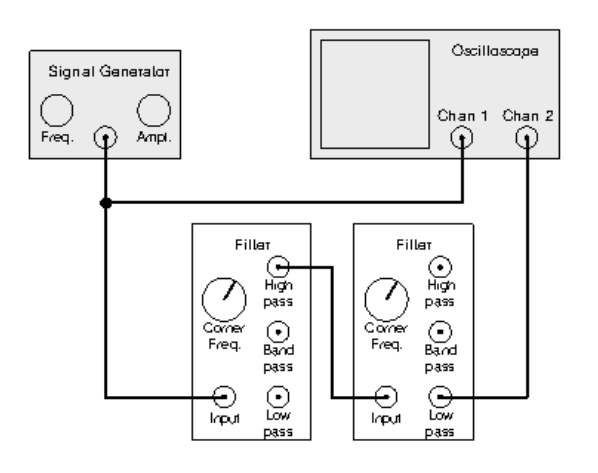
\includegraphics[width=.5\textwidth]{425_schaltplan_bandpass.png}
	\caption{Schaltplan des Bandpass.\cite{anleitung425}} \label{fig:schaltplan_bandpass}
\end{figure}

Die effektive Bandbreite wird mit der Verstärkung
\begin{align}
	G(f)=\dfrac{V^\textsc{rms}_\text{output}}{V^\textsc{rms}_\text{input}}
\end{align}
bestimmt
\begin{align}
	\Delta f_\text{eff}=\int_{0}^{\infty}\td fG^2(f)=\int_{0}^{\infty}\td fG_\text{LP}^2(f)G_\text{HP}^2(f)
	,\end{align}
mit der Tiefpassverstärkung $G_\text{LP}(f)=\left(1+(f/f_\text{l})^4\right)^{-1/2}$ und der Hochpassverstärkung $G_\text{HP}\left(f\right)=\left(f/f_\text{h}\right)^2\left(1+(f/f_\text{h})^4\right)^{-1/2}$.
$f_\text{h}$ und $f_\text{l}$ sind die eingestellten Grenzfrequenzen von Hoch-- und Tiefpass.
Das analytische Ergebnis des Integrals ist
\begin{align}
	\Delta f_\text{eff}=\dfrac{f_\text{l}^4\pi \left(f_\text{h}-f_\text{l}\right)}{2^{3/2}\left(f_\text{h}^4-f_\text{l}^4\right)}
	.\end{align}

\subsection{Durchführung \& Auswertung} \label{sec:bandbreite}
Die Bandbreite wird für $f_\text{h}=\SI{100}{Hz}$ und $f_\text{l}=\SI{10}{kHz}$ bestimmt.
Mit dem Frequenzgenerator werden, für eine konstante Eingangsspannung, verschiedene Frequenzen von $\SI{2}{Hz}$ bis $\SI{8}{MHz}$ eingestellt und die Ausgangsspannung gemessen. Es ergeben sich die Werte aus Tab. \ref{tab:frequency_data}.
Daraus bestimmt sich jeweils die Grenzfrequenz und damit die Bandbreite.

Abb.\ (\ref{fig:bandpass}) zeigt die Verstärkung gegen die eingestellte Frequenz. Es ist gut zu erkennen, dass die Verstärkung um die eingestellen Frequenzen von \SI{100}{Hz} und \SI{10}{\kilo Hz} zwei Wendepunkte aufweist.
Aus Abb.\ (\ref{fig:bandpass}) lassen sich auch die Grenzfrequenzen von Hoch-- und Tiefpass bestimmen. Für die Anpassungen werden die respektiven Gleichungen zur Verstärkung verwendet. 
Diese sind in Tab.\ (\ref{tab:bandpass_parameter}) eingetragen. Da $\chi^2/\text{ddof}=\SI{0.047}{}$ deutlich unter dem optimalen Wert von 1 liegt, kann davon ausgegangen werden, dass die Messunsicherheit zu groß eingeschätzt wurde.
Sie stimmen mit den eingestellten Frequenzen überein und die resultierende Bandbreite ist die Differenz zwischen den Grenzfrequenzen.

\begin{figure}[t]
	\centering
	\resizebox{.5\textwidth}{!}{% GNUPLOT: LaTeX picture with Postscript
\begingroup
  \makeatletter
  \providecommand\color[2][]{%
    \GenericError{(gnuplot) \space\space\space\@spaces}{%
      Package color not loaded in conjunction with
      terminal option `colourtext'%
    }{See the gnuplot documentation for explanation.%
    }{Either use 'blacktext' in gnuplot or load the package
      color.sty in LaTeX.}%
    \renewcommand\color[2][]{}%
  }%
  \providecommand\includegraphics[2][]{%
    \GenericError{(gnuplot) \space\space\space\@spaces}{%
      Package graphicx or graphics not loaded%
    }{See the gnuplot documentation for explanation.%
    }{The gnuplot epslatex terminal needs graphicx.sty or graphics.sty.}%
    \renewcommand\includegraphics[2][]{}%
  }%
  \providecommand\rotatebox[2]{#2}%
  \@ifundefined{ifGPcolor}{%
    \newif\ifGPcolor
    \GPcolortrue
  }{}%
  \@ifundefined{ifGPblacktext}{%
    \newif\ifGPblacktext
    \GPblacktexttrue
  }{}%
  % define a \g@addto@macro without @ in the name:
  \let\gplgaddtomacro\g@addto@macro
  % define empty templates for all commands taking text:
  \gdef\gplbacktext{}%
  \gdef\gplfronttext{}%
  \makeatother
  \ifGPblacktext
    % no textcolor at all
    \def\colorrgb#1{}%
    \def\colorgray#1{}%
  \else
    % gray or color?
    \ifGPcolor
      \def\colorrgb#1{\color[rgb]{#1}}%
      \def\colorgray#1{\color[gray]{#1}}%
      \expandafter\def\csname LTw\endcsname{\color{white}}%
      \expandafter\def\csname LTb\endcsname{\color{black}}%
      \expandafter\def\csname LTa\endcsname{\color{black}}%
      \expandafter\def\csname LT0\endcsname{\color[rgb]{1,0,0}}%
      \expandafter\def\csname LT1\endcsname{\color[rgb]{0,1,0}}%
      \expandafter\def\csname LT2\endcsname{\color[rgb]{0,0,1}}%
      \expandafter\def\csname LT3\endcsname{\color[rgb]{1,0,1}}%
      \expandafter\def\csname LT4\endcsname{\color[rgb]{0,1,1}}%
      \expandafter\def\csname LT5\endcsname{\color[rgb]{1,1,0}}%
      \expandafter\def\csname LT6\endcsname{\color[rgb]{0,0,0}}%
      \expandafter\def\csname LT7\endcsname{\color[rgb]{1,0.3,0}}%
      \expandafter\def\csname LT8\endcsname{\color[rgb]{0.5,0.5,0.5}}%
    \else
      % gray
      \def\colorrgb#1{\color{black}}%
      \def\colorgray#1{\color[gray]{#1}}%
      \expandafter\def\csname LTw\endcsname{\color{white}}%
      \expandafter\def\csname LTb\endcsname{\color{black}}%
      \expandafter\def\csname LTa\endcsname{\color{black}}%
      \expandafter\def\csname LT0\endcsname{\color{black}}%
      \expandafter\def\csname LT1\endcsname{\color{black}}%
      \expandafter\def\csname LT2\endcsname{\color{black}}%
      \expandafter\def\csname LT3\endcsname{\color{black}}%
      \expandafter\def\csname LT4\endcsname{\color{black}}%
      \expandafter\def\csname LT5\endcsname{\color{black}}%
      \expandafter\def\csname LT6\endcsname{\color{black}}%
      \expandafter\def\csname LT7\endcsname{\color{black}}%
      \expandafter\def\csname LT8\endcsname{\color{black}}%
    \fi
  \fi
    \setlength{\unitlength}{0.0500bp}%
    \ifx\gptboxheight\undefined%
      \newlength{\gptboxheight}%
      \newlength{\gptboxwidth}%
      \newsavebox{\gptboxtext}%
    \fi%
    \setlength{\fboxrule}{0.5pt}%
    \setlength{\fboxsep}{1pt}%
    \definecolor{tbcol}{rgb}{1,1,1}%
\begin{picture}(7200.00,4320.00)%
    \gplgaddtomacro\gplbacktext{%
      \csname LTb\endcsname%%
      \put(731,619){\makebox(0,0)[r]{\strut{}$-0.2$}}%
      \csname LTb\endcsname%%
      \put(731,1117){\makebox(0,0)[r]{\strut{}$0$}}%
      \csname LTb\endcsname%%
      \put(731,1615){\makebox(0,0)[r]{\strut{}$0.2$}}%
      \csname LTb\endcsname%%
      \put(731,2113){\makebox(0,0)[r]{\strut{}$0.4$}}%
      \csname LTb\endcsname%%
      \put(731,2611){\makebox(0,0)[r]{\strut{}$0.6$}}%
      \csname LTb\endcsname%%
      \put(731,3110){\makebox(0,0)[r]{\strut{}$0.8$}}%
      \csname LTb\endcsname%%
      \put(731,3608){\makebox(0,0)[r]{\strut{}$1$}}%
      \csname LTb\endcsname%%
      \put(731,4106){\makebox(0,0)[r]{\strut{}$1.2$}}%
      \csname LTb\endcsname%%
      \put(829,425){\makebox(0,0){\strut{}$1$}}%
      \csname LTb\endcsname%%
      \put(1695,425){\makebox(0,0){\strut{}$10$}}%
      \csname LTb\endcsname%%
      \put(2560,425){\makebox(0,0){\strut{}$100$}}%
      \csname LTb\endcsname%%
      \put(3425,425){\makebox(0,0){\strut{}$1000$}}%
      \csname LTb\endcsname%%
      \put(4290,425){\makebox(0,0){\strut{}$10000$}}%
      \csname LTb\endcsname%%
      \put(5155,425){\makebox(0,0){\strut{}$100000$}}%
      \csname LTb\endcsname%%
      \put(6021,425){\makebox(0,0){\strut{}$1\times10^{6}$}}%
      \csname LTb\endcsname%%
      \put(6886,425){\makebox(0,0){\strut{}$1\times10^{7}$}}%
    }%
    \gplgaddtomacro\gplfronttext{%
      \csname LTb\endcsname%%
      \put(170,2362){\rotatebox{-270}{\makebox(0,0){\strut{}$G$}}}%
      \csname LTb\endcsname%%
      \put(3858,135){\makebox(0,0){\strut{}$f/\SI{}{Hz}$}}%
      \csname LTb\endcsname%%
      \put(6123,3932){\makebox(0,0)[r]{\strut{}Hochpass Dominiert}}%
      \csname LTb\endcsname%%
      \put(6123,3738){\makebox(0,0)[r]{\strut{}Tiefpass Dominiert}}%
      \csname LTb\endcsname%%
      \put(6123,3545){\makebox(0,0)[r]{\strut{}Hochpass Modell $G_{\text{HP}}(f)$}}%
      \csname LTb\endcsname%%
      \put(6123,3351){\makebox(0,0)[r]{\strut{}Tiefpass Modell $G_{\text{LP}}(f)$}}%
    }%
    \gplbacktext
    \put(0,0){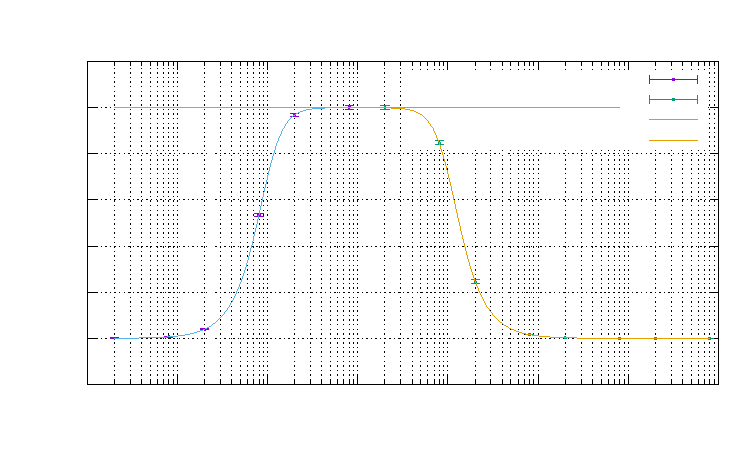
\includegraphics[width={360.00bp},height={216.00bp}]{eff_band}}%
    \gplfronttext
  \end{picture}%
\endgroup
}
	\caption{Gemessene Verstärkung $G=\frac{U_{\textsc{rms}}}{U_{0\textsc{, rms}}}$ im Bandpass.} \label{fig:bandpass}
\end{figure}
\begin{table}[t]
	\begin{tabular}{cc}
		\toprule
		\textbf{Parameter} & {\textbf{Wert(Fehler)}} \\
		\midrule
		$f_l$              & \SI{10104 \pm 56}{Hz}     \\
		$f_h$              & \SI{100.50 \pm 0.17}{Hz}  \\
		\bottomrule
	\end{tabular}
	\label{tab:bandpass_parameter}
	\caption{Frequenzabhängigkeit modelliert mit $G_\text{LP}(f)=\left[1+(f/f_l)^4\right]^{-1/2}$ und $G_\text{HP}(f)=(f/f_h)^2\left[1+(f/f_h)^4\right]^{-1/2}$}
\end{table}
Die Bandbreite berechnet sich dann zu
\begin{align}
	\Delta f_\text{eff}\approx \SI{11109+-60}{Hz}[1\%]
	.\end{align}
Der errechnete Wert und dessen Unsicherheit liegen in dem erwartetem Bereich von etwa \SI{10}{\kilo Hz}.
\section{\textsc{Johnson}--Rauschen}
\subsection{Theoretischer Hintergrund}
Das \textsc{Johnson}--Rauschen, auch thermisches Rauschen, entsteht durch thermodynamische Fluktuationen der Elektronen im Leitungsband.
Dies geschieht, im Vergleich zum Schrotrauschen, ohne, dass eine Spannung angelegt ist.
Elektronen bewegen sich im thermischen Gleichgewicht ungeordnet aufgrund ihrer thermischen Energie wodurch sie kurze Spannungs-- bzw.\ Strompulse erzeugen.
Mit Hilfe von sensitiven Messgeräten kann dieses Rauschen untersucht werden.

Der formale Zusammenhang der mittleren quadratischen Rauschspannung in einem Widerstand $R$ ist
\begin{align}
	\overline{V^2_\text{J}}=4k_\text{B}TR\Delta f_\text{eff}
	,\end{align}
mit der Temperatur $T$ und der Bandbreite $\Delta f_\text{eff}$.

\subsection{Durchführung \& Auswertung: Beobachtung des \textsc{Johnson}--Rauschens}
Das \textsc{Johnson}--Rauschen wird im Vorverstärkerschaltkreis aus Abb.\ (\ref{fig:vorverstärker}) beobachtet.
Diese Schaltung befand sich in der LLE--Box Abb.\ (\ref{fig:johnson_lle}), welche entsprechend verkabelt werden musste.
Zur Beobachtung wurden folgende Werte eingestellt
\begin{align}
	R_\text{in}=\SI{100}{k\ohm},R_\text{f}=\SI{1}{k\ohm}
	.\end{align}
Die LLE--Box wurde dann mit der HLE--Box Abb.\ (\ref{fig:johnson_hle}) verbunden.
Die Einstellung der HLE--Box war
\begin{align}
	f_\text{h}=\SI{.1}{kHz},f_\text{l}=\SI{100}{kHz},\text{Gain}=300,\text{AC}
	.\end{align}
Das Rauschen ließ sich dann auf dem Oszillographen beobachten Abb.\ (\ref{fig:johnson_oszi}).
Es ist klar zu erkennen, dass das Rauschen starken Fluktuationen unterliegt und ungeordnet ist.
Im Mittel bleibt es allerdings konstant.

\begin{figure}[t]
	\centering
	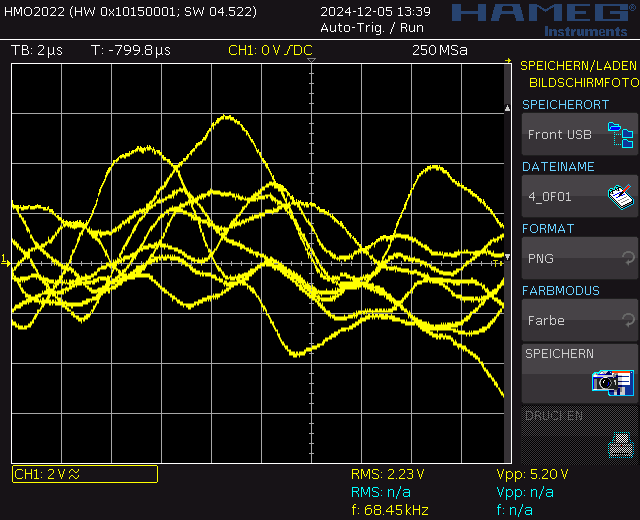
\includegraphics[width=.5\textwidth]{../data/4_0F01.png}
	\caption{Oszillogramm des \textsc{Johnson}--Rauschen.} \label{fig:johnson_oszi}
\end{figure}

\begin{figure}[t]
	\centering
	\includegraphics[width=.5\textwidth]{425_schaltplan_vorverstärker_LLE.png}
	\caption{Vorverstärkerschaltkreis zur Beobachtung des \textsc{Johnson}--Rauschens.\cite{anleitung425}} \label{fig:vorverstärker}
\end{figure}

\begin{figure}[t]
	\centering
	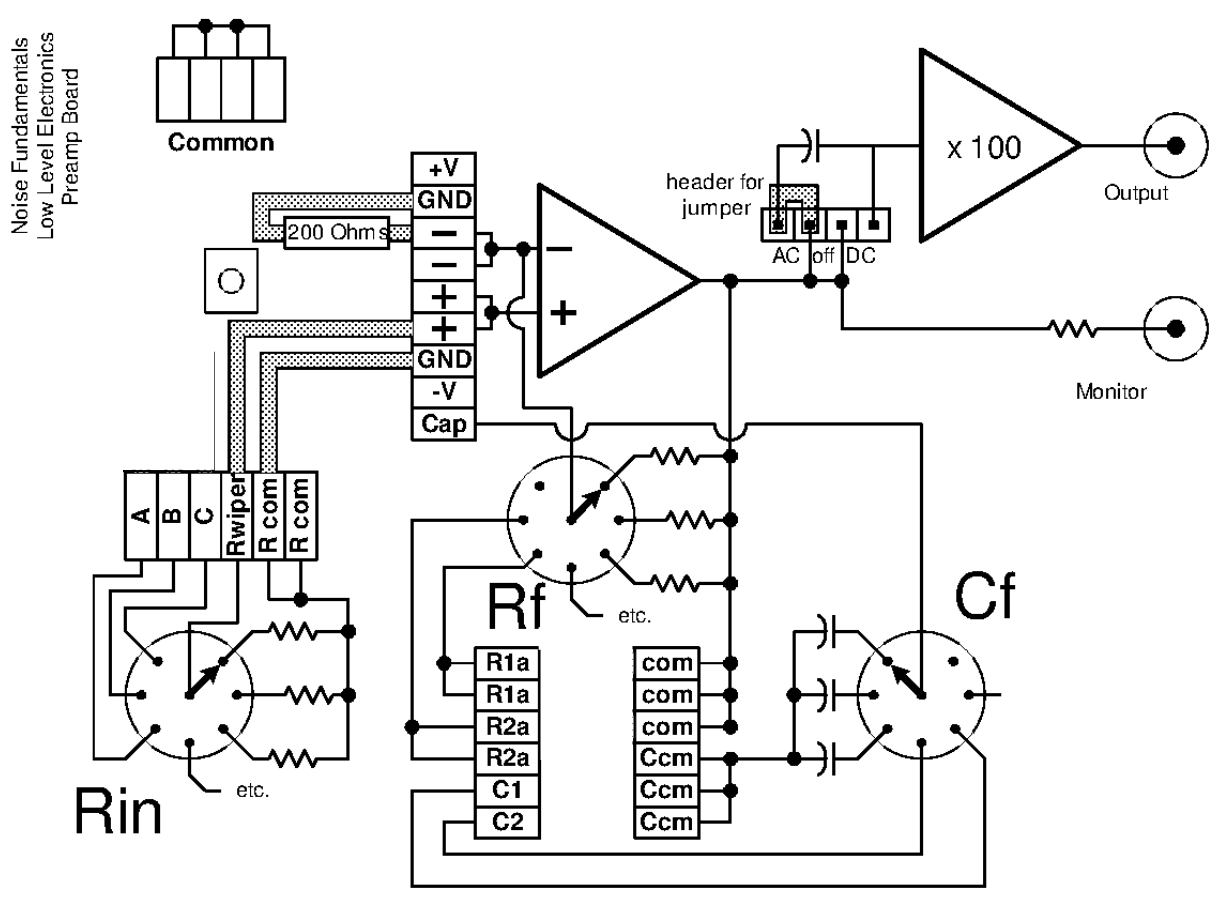
\includegraphics[width=.5\textwidth]{425_schaltplan_johnson_LLE.png}
	\caption{Die LLE--Box zur Messung und Beobachtung des \textsc{Johnson}--Rauschens.\cite{anleitung425}} \label{fig:johnson_lle}
\end{figure}

\begin{figure}[t]
	\centering
	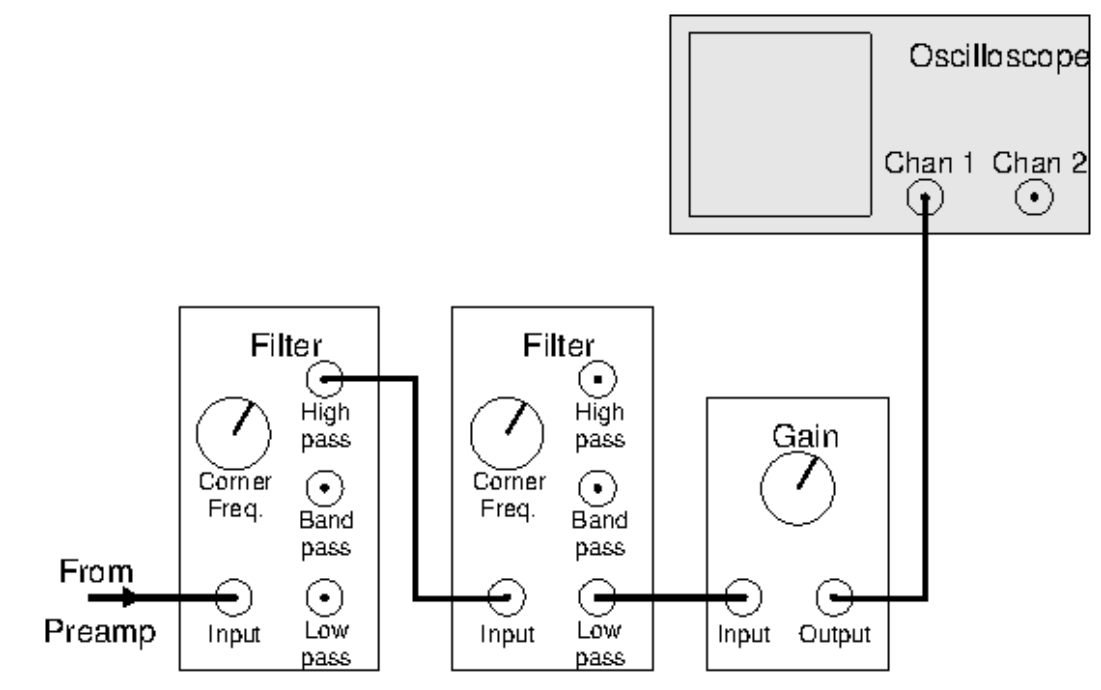
\includegraphics[width=.5\textwidth]{425_schaltplan_visualisierung_johnson_HLE.png}
	\caption{HLE--Box zur Messung und Beobachtung des \textsc{Johnson}--Rauschens.\cite{anleitung425}} \label{fig:johnson_hle}
\end{figure}

\subsection{Durchführung \& Auswertung: Messung des \textsc{Johnson}--Rauschens}
Zur Messung der mittleren Spannung des Rauschens wird die Schaltung aus Abb.\ (\ref{fig:johnson_hle_messung}) verwendet.
Die Einstellungen waren zusätzlich
\begin{align}
	\text{Multiplier}:\text{A}\times \text{A},\text{Zeitkonst.}=\SI{1}{s}
	.\end{align}
Durch den Multiplier ist das Ausgangssignal der HLE--Box
\begin{align}
	V_\text{out}=\dfrac{\overline{\left(V_\text{in}(t)\right)^2}}{\SI{10}{V}}
	.\end{align}
Dieses Signal wird dann über die Zeitkonstante von $\SI{1}{s}$ gemittelt.

Um zu überprüfen, ob der Multiplier wie erwartet funktioniert, kann der Output der HLE--Box gegen den Multiplier aufgetragen werden.
Es ergibt sich Abb.\ (\ref{fig:multiplier}).
Der quadratische Zusammenhang mit Verschiebung ist klar zu erkennen. Dieser ensteht aufgrund der Verstärkung und Quadrierung des Multipliers nach Formel (9). Erst nach dem Multiplier wird das Signal zeitlich gemittelt.% TODO: Warum?

Da das Ausgangssignal nur in einem kleinen Bereich -- zwischen $\SI{0.6}{V}$ und $\SI{1.2}{V}$ -- stabil und linear zum Eingangsrauschen ist, wird das DMM mit Hilfe der Verstärkung in diesem Bereich gehalten.
Der Zusammenhang zwischen der am DMM abgelesenen Spannung ist modelliert durch
\begin{align}
	V_\text{meter}=\overline{V_\text{J}^2(t)+V_\text{N}^2(t)}\dfrac{\left(600G_2\right)^2}{\SI{10}{V}}
	,\end{align}
wobei das Rauschen in die beiden Anteile $V_\text{J}$ und $V_\text{N}$ aufgeteilt werden muss.
$V_\text{J}$ ist das \textsc{Johnson}--Rauschen und $V_\text{N}$ ist der Anteil des Rauschens, der innerhalb der Verstärker entsteht.
Eine Korrelation zwischen diesen beiden Rauschtypen gibt es nicht, da sie auf unterschiedlichen Phänomenen beruhen.
Das \textsc{Johnson}--Rauschen ist abhängig von der Temperatur und dem Widerstand, das Verstärkerrauschen nicht.
Diese Tatsache erlaubt daher die Bestimmung von $V_\text{J}$ über die Variation des Widerstands $R_\text{in}$ (da $V_\text{J}=V_\text{J}(R_\text{in})$ und $V_\text{N}\neq V_\text{N}(R_\text{in})$).
Das \textsc{Johnson}--Rauschen kann zusätzlich über die Variation der Bandbreite erfolgen, da es von der Verstärkung $G_2$ abhängt.

\begin{figure}[t]
	\centering
	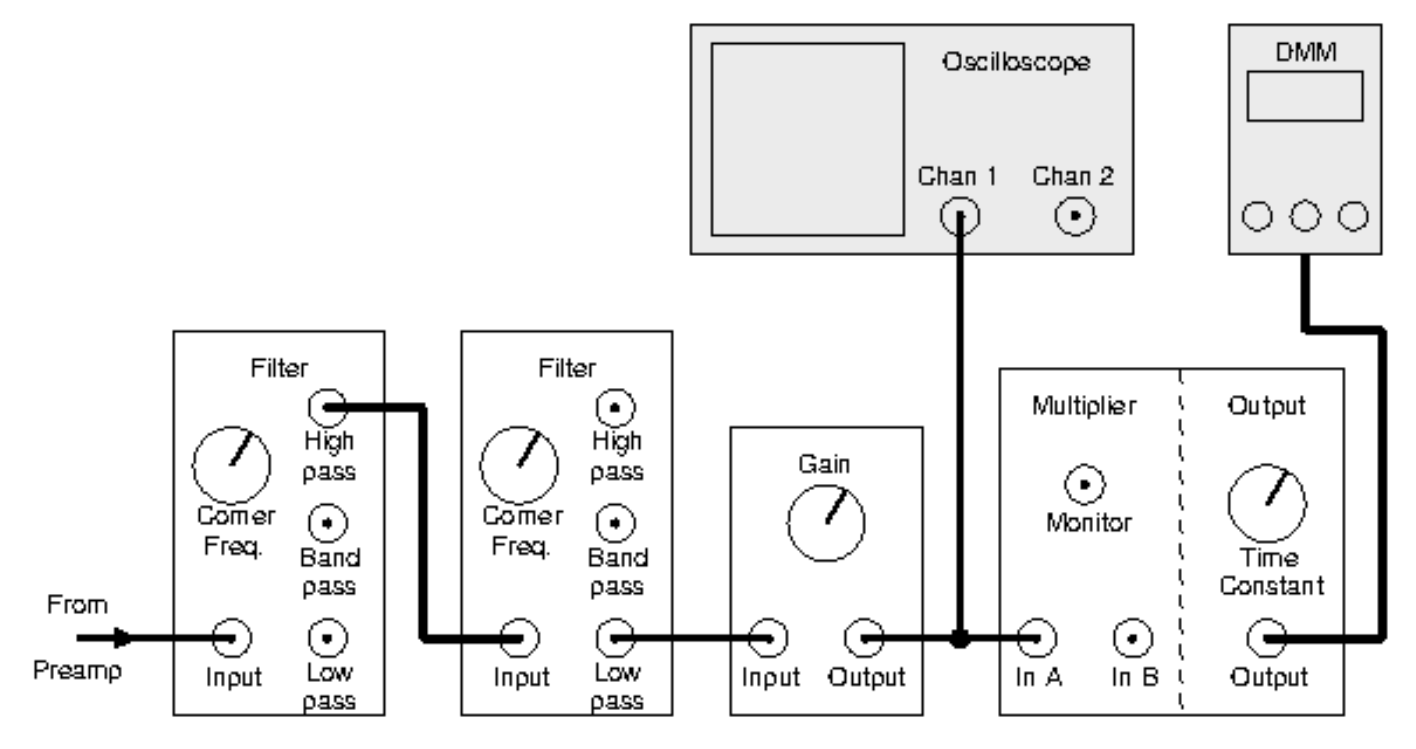
\includegraphics[width=.5\textwidth]{425_schaltplan_messung_johnson.png}
	\caption{HLE--Box zur Messung des \textsc{Johnson}--Rauschens.\cite{anleitung425}} \label{fig:johnson_hle_messung}
\end{figure}

\begin{figure}[t]
	\centering
	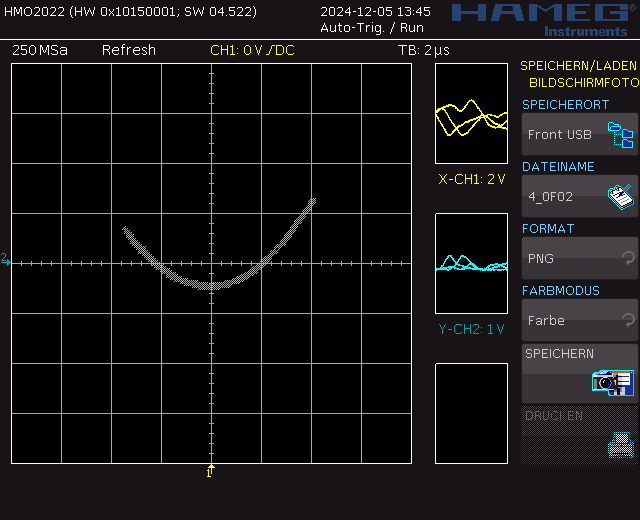
\includegraphics[width=.5\textwidth]{../data/4_0F02.png}
	\caption{Output der HLE--Box (Kanal 1) gegen Multiplier (Kanal 2).} \label{fig:multiplier}
\end{figure}

\subsubsection{Variation des Widerstands}
Wird der Widerstand variiert, um so das \textsc{Johnson}--Rauschen zu bestimmen, ergeben sich Abb.\ (\ref{fig:johnson_widerstand_messung}) mit Tab.\ (\ref{tab:johnson_widerstand_parameter}). Die ursprünglichen Messwerte sind in Tab. (\ref{tab:john_wid}).

Da $\chi^2/\text{ddof}=\SI{39.749}{}$, kann davon ausgegangen werden, dass in diesem Fall die Messunsicherheit unterschätzt wurde.

Der Messpunkt für den größten Widerstand bei \SI{1}{\mega \Omega} folgt offensichtlich nicht dem linearen Verhalten der restlichen Datenpunkte, insofern wird dieser Punkt für die Anpassung ausgelassen.

Es lässt sich an der Darstellung der Residuen Abb.\ (\ref{fig:residuen}) erkennen, dass sie mit größer werdendem Widerstand steigen, was bedeutet, dass das lineare Verhalten für große Widerstände nicht passend ist. Dies ist besonders für die letzten drei Werte ersichtlich, da dessen Messunsicherheit nicht mehr die x-Achse schneiden, also nicht mit dem Funktional übereinstimmmen.

\begin{figure}[t]
	\centering
	\resizebox{.5\textwidth}{!}{\input{Widerstandsabhängigkeit.tex}}
	\caption{Widerstandsabhängigkeit mit $\overline{V_J^2(t)+V_N^2(t)}=V_{\text{meter}}\frac{\SI{10}{V}}{(600\cdot G_2)^2}$} \label{fig:johnson_widerstand_messung}
\end{figure}
\begin{table}[t]
	\begin{tabular}{cc}
		\toprule
		\textbf{Parameter} & {\textbf{Wert(Fehler)}}  \\
		\midrule
		m                  & \SI{1.51 \pm 0.11e-15}{V^2 \per \Omega} \\
		b                  & \SI{7.04 \pm 0.29e-12}{V^2} \\
		\bottomrule
	\end{tabular}
	\label{tab:johnson_widerstand_parameter}
	\caption{Widerstandsabhängigkeit modelliert mit $\overline{V_J^2(t)+V_N^2(t)}(R_\text{in})=m\cdot R+b$}
\end{table}
\begin{figure}[t]
	\centering
	\resizebox{.5\textwidth}{!}{% GNUPLOT: LaTeX picture with Postscript
\begingroup
  \makeatletter
  \providecommand\color[2][]{%
    \GenericError{(gnuplot) \space\space\space\@spaces}{%
      Package color not loaded in conjunction with
      terminal option `colourtext'%
    }{See the gnuplot documentation for explanation.%
    }{Either use 'blacktext' in gnuplot or load the package
      color.sty in LaTeX.}%
    \renewcommand\color[2][]{}%
  }%
  \providecommand\includegraphics[2][]{%
    \GenericError{(gnuplot) \space\space\space\@spaces}{%
      Package graphicx or graphics not loaded%
    }{See the gnuplot documentation for explanation.%
    }{The gnuplot epslatex terminal needs graphicx.sty or graphics.sty.}%
    \renewcommand\includegraphics[2][]{}%
  }%
  \providecommand\rotatebox[2]{#2}%
  \@ifundefined{ifGPcolor}{%
    \newif\ifGPcolor
    \GPcolortrue
  }{}%
  \@ifundefined{ifGPblacktext}{%
    \newif\ifGPblacktext
    \GPblacktexttrue
  }{}%
  % define a \g@addto@macro without @ in the name:
  \let\gplgaddtomacro\g@addto@macro
  % define empty templates for all commands taking text:
  \gdef\gplbacktext{}%
  \gdef\gplfronttext{}%
  \makeatother
  \ifGPblacktext
    % no textcolor at all
    \def\colorrgb#1{}%
    \def\colorgray#1{}%
  \else
    % gray or color?
    \ifGPcolor
      \def\colorrgb#1{\color[rgb]{#1}}%
      \def\colorgray#1{\color[gray]{#1}}%
      \expandafter\def\csname LTw\endcsname{\color{white}}%
      \expandafter\def\csname LTb\endcsname{\color{black}}%
      \expandafter\def\csname LTa\endcsname{\color{black}}%
      \expandafter\def\csname LT0\endcsname{\color[rgb]{1,0,0}}%
      \expandafter\def\csname LT1\endcsname{\color[rgb]{0,1,0}}%
      \expandafter\def\csname LT2\endcsname{\color[rgb]{0,0,1}}%
      \expandafter\def\csname LT3\endcsname{\color[rgb]{1,0,1}}%
      \expandafter\def\csname LT4\endcsname{\color[rgb]{0,1,1}}%
      \expandafter\def\csname LT5\endcsname{\color[rgb]{1,1,0}}%
      \expandafter\def\csname LT6\endcsname{\color[rgb]{0,0,0}}%
      \expandafter\def\csname LT7\endcsname{\color[rgb]{1,0.3,0}}%
      \expandafter\def\csname LT8\endcsname{\color[rgb]{0.5,0.5,0.5}}%
    \else
      % gray
      \def\colorrgb#1{\color{black}}%
      \def\colorgray#1{\color[gray]{#1}}%
      \expandafter\def\csname LTw\endcsname{\color{white}}%
      \expandafter\def\csname LTb\endcsname{\color{black}}%
      \expandafter\def\csname LTa\endcsname{\color{black}}%
      \expandafter\def\csname LT0\endcsname{\color{black}}%
      \expandafter\def\csname LT1\endcsname{\color{black}}%
      \expandafter\def\csname LT2\endcsname{\color{black}}%
      \expandafter\def\csname LT3\endcsname{\color{black}}%
      \expandafter\def\csname LT4\endcsname{\color{black}}%
      \expandafter\def\csname LT5\endcsname{\color{black}}%
      \expandafter\def\csname LT6\endcsname{\color{black}}%
      \expandafter\def\csname LT7\endcsname{\color{black}}%
      \expandafter\def\csname LT8\endcsname{\color{black}}%
    \fi
  \fi
    \setlength{\unitlength}{0.0500bp}%
    \ifx\gptboxheight\undefined%
      \newlength{\gptboxheight}%
      \newlength{\gptboxwidth}%
      \newsavebox{\gptboxtext}%
    \fi%
    \setlength{\fboxrule}{0.5pt}%
    \setlength{\fboxsep}{1pt}%
    \definecolor{tbcol}{rgb}{1,1,1}%
\begin{picture}(7200.00,4320.00)%
    \gplgaddtomacro\gplbacktext{%
      \csname LTb\endcsname%%
      \put(634,619){\makebox(0,0)[r]{\strut{}$-50$}}%
      \csname LTb\endcsname%%
      \put(634,1117){\makebox(0,0)[r]{\strut{}$0$}}%
      \csname LTb\endcsname%%
      \put(634,1615){\makebox(0,0)[r]{\strut{}$50$}}%
      \csname LTb\endcsname%%
      \put(634,2113){\makebox(0,0)[r]{\strut{}$100$}}%
      \csname LTb\endcsname%%
      \put(634,2611){\makebox(0,0)[r]{\strut{}$150$}}%
      \csname LTb\endcsname%%
      \put(634,3110){\makebox(0,0)[r]{\strut{}$200$}}%
      \csname LTb\endcsname%%
      \put(634,3608){\makebox(0,0)[r]{\strut{}$250$}}%
      \csname LTb\endcsname%%
      \put(634,4106){\makebox(0,0)[r]{\strut{}$300$}}%
      \csname LTb\endcsname%%
      \put(731,425){\makebox(0,0){\strut{}$1$}}%
      \csname LTb\endcsname%%
      \put(1757,425){\makebox(0,0){\strut{}$10$}}%
      \csname LTb\endcsname%%
      \put(2783,425){\makebox(0,0){\strut{}$100$}}%
      \csname LTb\endcsname%%
      \put(3809,425){\makebox(0,0){\strut{}$1000$}}%
      \csname LTb\endcsname%%
      \put(4834,425){\makebox(0,0){\strut{}$10000$}}%
      \csname LTb\endcsname%%
      \put(5860,425){\makebox(0,0){\strut{}$100000$}}%
      \csname LTb\endcsname%%
      \put(6886,425){\makebox(0,0){\strut{}$1\times10^{6}$}}%
    }%
    \gplgaddtomacro\gplfronttext{%
      \csname LTb\endcsname%%
      \put(170,2362){\rotatebox{-270}{\makebox(0,0){\strut{}$\text{res}/\SI{}{\micro V^2}$}}}%
      \csname LTb\endcsname%%
      \put(3809,135){\makebox(0,0){\strut{}$R/\SI{}{\Omega}$}}%
      \csname LTb\endcsname%%
      \put(6123,793){\makebox(0,0)[r]{\strut{}Residuen}}%
    }%
    \gplbacktext
    \put(0,0){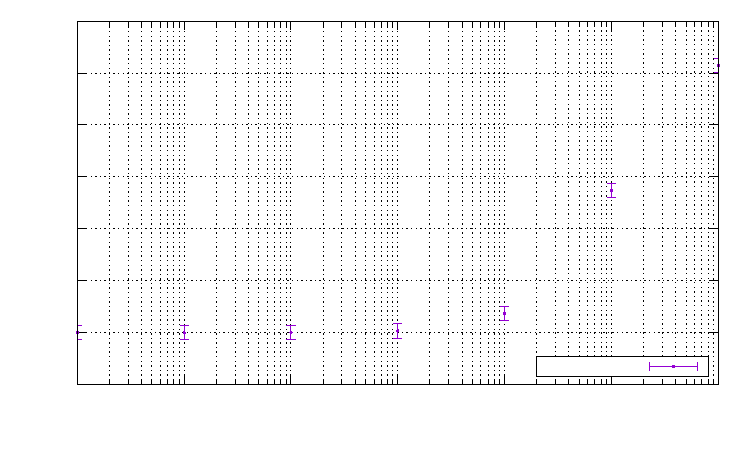
\includegraphics[width={360.00bp},height={216.00bp}]{Widerstandsresiduen}}%
    \gplfronttext
  \end{picture}%
\endgroup
}
	\caption{Die Residuen zur Widerstandsabhängigkeit; $\text{res}=\overline{u^2}-\hat{\overline{u^2}}$.} \label{fig:residuen}
\end{figure}
Aufgrund der \textsc{Nyquist}--Formel kann man das gesamte und auch insbesondere das \textsc{Johnson}--Rauschen folgendermaßen identifizieren
\begin{align}
	\overline{V_\text{J}^2+V_\text{N}^2}=4k_B^RRT\Delta f_\text{eff}+\overline{V_\text{N}^2}
	.\end{align}
Aus der Anpassung geht hervor
\begin{align}
	\overline{V_\text{J}^2+V_\text{N}^2}=mR+b
	,\end{align}
sodass
\begin{align}
	k_B^R=\dfrac{m}{4T\Delta f_\text{eff}}\qquad \overline{V_\text{N}^2}=b
	.\end{align}
Die Temperatur war $T=\SI{293.95+-0.5}{K}$ und die Bandbreite $\Delta f_\text{eff}\approx \SI{11109+-60}{Hz}$.
Damit ist die \textsc{Boltzmann}--Konstante
\begin{align}
	k_B^R          & =\SI{11.53+-0.09e-23}{J/K}[1\%,112.7\sigma] \\
	k_B^\text{lit} & =\SI{1.380e-23}{J/K}
\end{align}
Der Literaturwert ist entnommen von CODATA\cite{codataBoltzmann}.
Die Abweichung dieses Werts von der Literatur ist sehr groß, da aber der relative Fehler sehr klein ist, deutet dies auf einen systematischen Fehler und nicht auf statistische Unsicherheiten hin.
Eine Ursache waren überraschenderweise Gräusche -- wie Dialog oder das Tippen auf der Tastatur -- die dazu geführt haben, dass sich die gemessenen Spannungen änderten.
Da dieses Phänomen nicht erwartet war, ist davon auszugehen, dass es weitere Ursachen gibt, deren Ursprung nicht klar ist.

Für die Durchführung ist somit die \textsc{Nyquist}--Formel nicht mit der Messung kompatibel.

\subsubsection{Variation der Bandbreite}
Dieses Verfahren ist analog zur Variation des Widerstands.
Für den Widerstand wird der größtmögliche Widerstand verwendet, bei dem das Rauschen noch lineares Verhalten zeigt: $R_\text{in}=\SI{1}{k\ohm}$.
Dies bewirkt, dass das Gesamtrauschen vom \textsc{Johnson}--Rauschen dominiert wird.

Wird die Bandbreite variiert, um so das \textsc{Johnson}--Rauschen zu bestimmen, ergeben sich Abb.\ (\ref{fig:johnson_bandbreite_plot}) mit Tab.\ (\ref{tab:johnson_bandbreite_parameter}). Die urspünglichen Messenwerte sind Tab. (\ref{tab:john_freq}) zu entnehmen.

Da $\chi^2/\text{ddof}=\SI{6.923}{}$, wurden die Messunsicherheiten leicht überschätzt, sind aber noch im guten Rahmen, sodass sie als repräsentativ angesehen werden können.

Es lässt sich erkennen, dass das \textsc{Johnson}--Rauschen linear mit der Bandbreite steigt.
Mit zunahme der Bandbreite werden immer mehr Frequenzen hindurchgelassen. Da allerdings das Rauschen linear steigt, muss jede Frequenz einen gleichen Beitrag leisten. 
Daher ist die Verstärkung unabhängig von der Frequenz.
Das \textsc{Johnson}--Rauschen ist also weißes Rauschen. 
Gleichzeitig lässt sich die Linearität der \textsc{Nyquist}--Formel bestätigen.

\begin{figure}[h]
	\centering
	\resizebox{.5\textwidth}{!}{\input{Bandbreitenabhängigkeit.tex}}
	\caption{Bandbreitenabhängkeit mit $\overline{V_J^2(t)+V_N^2(t)}=V_{\text{meter}}\frac{\SI{10}{V}}{(600\cdot G_2)^2}$ und $\Delta f_{\text{eff}}=\frac{f_l^4\pi (f_l-f_h)}{2^{3/2}(f_l^4-f_h^4)}$} \label{fig:johnson_bandbreite_plot}
\end{figure}
\begin{table}[h!]
	\begin{tabular}{cc}
		\toprule
		\textbf{Parameter} & {\textbf{Wert(Fehler)}}    \\
		\midrule
		m                  & \SI{7.943 \pm 0.069e-17}{V^2\per Hz} \\
		b                  & \SI{7.5 \pm 4.5e-15}{V^2}     \\
		\bottomrule
	\end{tabular}
	\label{tab:parameter}
	\caption{Bandbreitenabhängigkeit modelliert mit $\overline{V_J^2(t)+V_N^2(t)}(\Delta f_{\text{eff}})=m\cdot \Delta f_{\text{eff}}+b$} \label{tab:johnson_bandbreite_parameter}
\end{table}
Es ist
\begin{align}
	\overline{V_\text{J}^2+V_\text{N}^2}=4k_B^fTR_\text{in}\Delta f_\text{eff}+\overline{V_\text{N}^2}
	.\end{align}
Aus der Anpassung geht hervor
\begin{align}
	\overline{V_\text{J}^2+V_\text{N}^2}=m\Delta f_\text{eff}+b
	,\end{align}
sodass
\begin{align}
	k_B^f=\dfrac{m}{4TR_\text{in}}\qquad \overline{V_\text{N}^2}=b
	.\end{align}
Der Widerstand lag bei $R_\text{in}=\SI{1}{k\ohm}$.
Damit ist die \textsc{Boltzmann}--Konstante
\begin{align}
	k_B^f          & =\SI{6.756+-0.06e-23}{J/K}[1\%,89.6\sigma] \\
	k_B^\text{lit} & =\SI{1.380e-23}{J/K}
\end{align}
Der Literaturwert ist entnommen von CODATA\cite{codataBoltzmann}.
Hier ist die Abweichung von der Literatur nicht so groß wie bei der Variation des Widerstands, es sind allerdings die selben Begründungen für die Abweichung.

Beide Verfahren liefern Werte, die sehr stark von der Literatur abweichen; $k_B^f$ ist näher an der Literatur als $k_B^R$.
Grund für den Unterschied zwischen $k_B^f$ und $k_B^R$ könnte sein, dass das \textsc{Johnson}--Rauschen weißes Rauschen ist -- daher unabhängig von der Frequenz -- aber abhängig von der Temperatur.
Das bedeutet, dass die Variation der Frequenz selbst keinen Einfluss hat, die Temperatur im Widerstand allerdings schon.
Deshalb ist die Abweichung bei der Frequenz geringer, da eine nicht unerhebliche Abweichung durch die Temperatur im Widerstand zustande kommen kann.
Die absolute Abweichung beider Verfahren von der Literatur sind dann auf systematische Fehler zurückzuführen. Diese wurden im vorigen Abschnitt diskutiert.

\section{Schrotrauschen}
\subsection{Theoretischer Hintergrund}
Da die elektrische Ladung in $e$ gequantelt ist, wird bei dem Übergang von Elektronen über eine Potentialbarriere (z.B.\ zwischen zwei Bauteilen, Photodiode, etc.) stets eine Ladung von genau einem $e$ transferiert.
Da die eingehende Ladung pro Zeit also nicht kontinuierlich ist, kommt es zu nicht stetigen Ausschlägen der Spannung, die über dieses Potential gemessen wird.
Diese Spannung wird als Schrotrauschen auf sensitiven Messgeräten wahrgenommen.

Formal ist das mittlere Rauschstromquadrat nach \textsc{Schottky}'s Formel:
\begin{align}
	\overline{\delta i^2}=2ei_\text{dc}\Delta f_\text{eff}
	,\end{align}
mit $i_\text{dc}$ der angelegten Stromstärke.
Da in der verwendeten Anordnung kein Hochpass verbaut ist, ist
\begin{align}
	\Delta f_\text{eff}=\int_{0}^{\infty}\td fG_\text{LP}^2\underbrace{G_\text{HP}^2}_{=1}=\dfrac{f_\text{l}\pi }{2^{3/2}}
	.\end{align}

\subsection{Durchführung \& Auswertung: Beobachtung des Schrotrauschens}
Das Schrotrauschen wurde innerhalb Abb.\ (\ref{fig:schrot_lle_beob}) bei einer Photodiode beobachtet.
Dafür wurde dieser Schaltkreis in Abb.\ (\ref{fig:schrot_lle_mess}) zusammengesteckt.
Die Elektronen aus der Photodiode wurden von einer Glühlampe herausgelöst, damit diese möglichst unkorreliert sind, um kein gleichmäßiges Rauschen zu erhalten.

Beobachtet wurde der Rauschstrom bzw.\ die Rauschspannung mit Abb.\ (\ref{fig:schaltplan_schrot_mess}).
Damit dies sichtbar war, wurde die Einstellung $f_\text{l}=\SI{100}{kHz}$ für die HLE--Box getroffen.
Es ergab sich ein ähnliches Bild zum \textsc{Johnson}--Rauschen. %TODO kein bild schrotrauschen beob??

\begin{figure}[t]
	\centering
	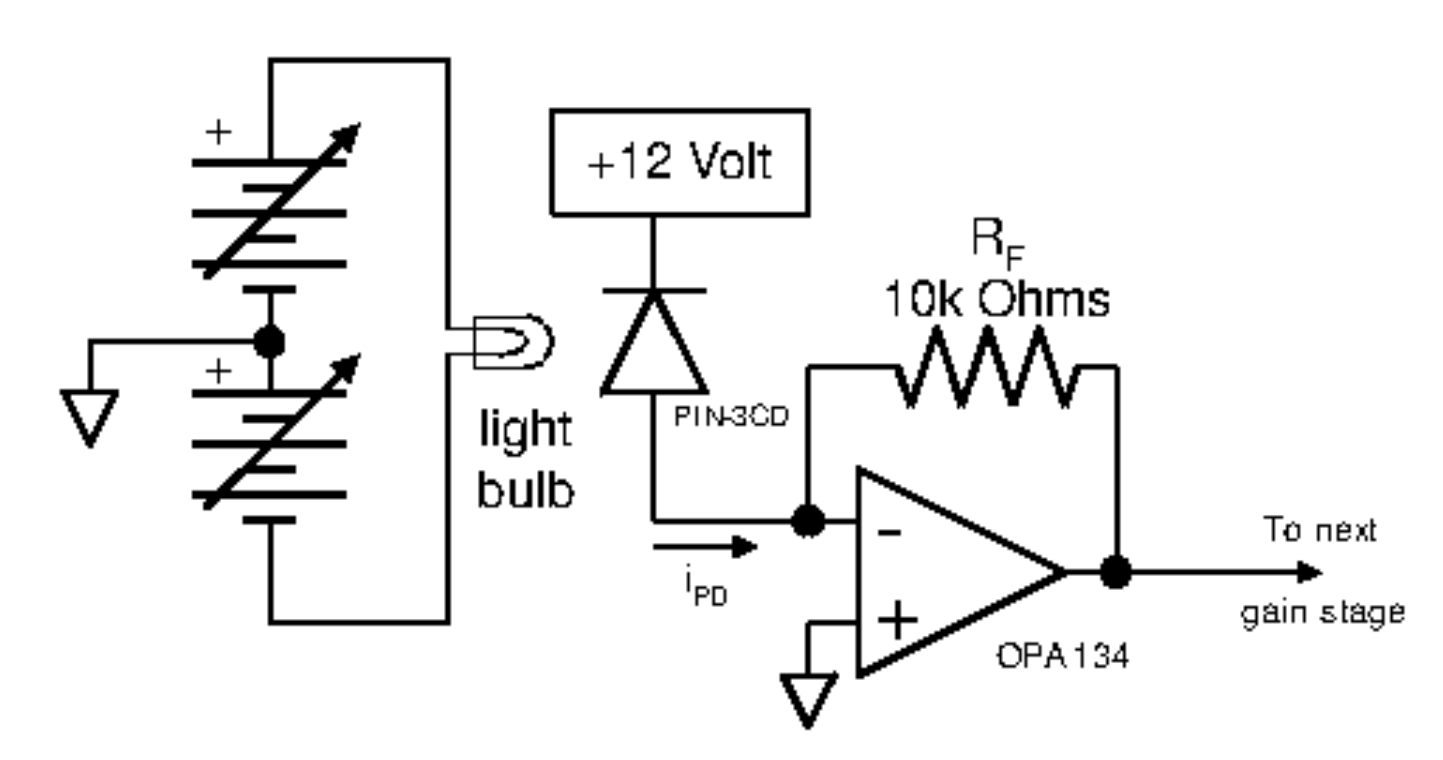
\includegraphics[width=.5\textwidth]{425_schaltplan_visualisierung_schort_LLE.png}
	\caption{Schaltung für die LLE--Box zur Beobachtung und Messung des Schrotrauschens.\cite{anleitung425}} \label{fig:schrot_lle_beob}
\end{figure}
\begin{figure}[t]
	\centering
	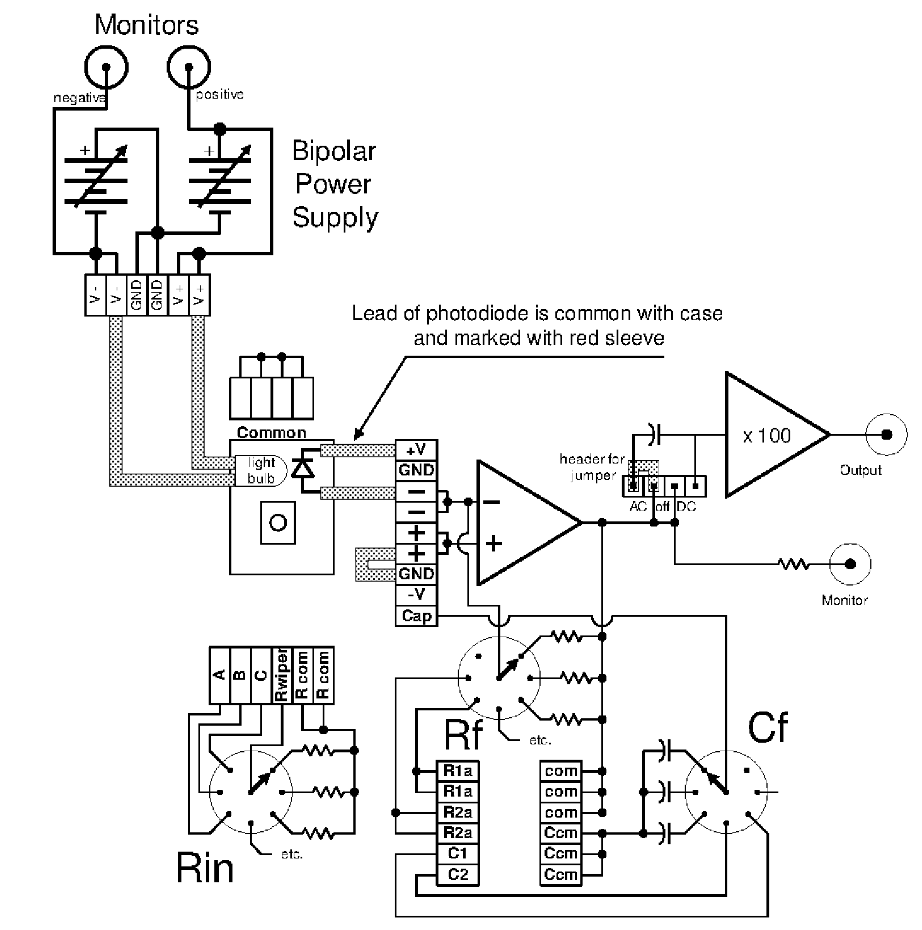
\includegraphics[width=.5\textwidth]{425_schaltplan_messung_schrot_LLE.png}
	\caption{LLE--Box zur Beobachtung und Messung des Schrotrauschens.\cite{anleitung425}} \label{fig:schrot_lle_mess}
\end{figure}
\begin{figure}[t]
	\centering
	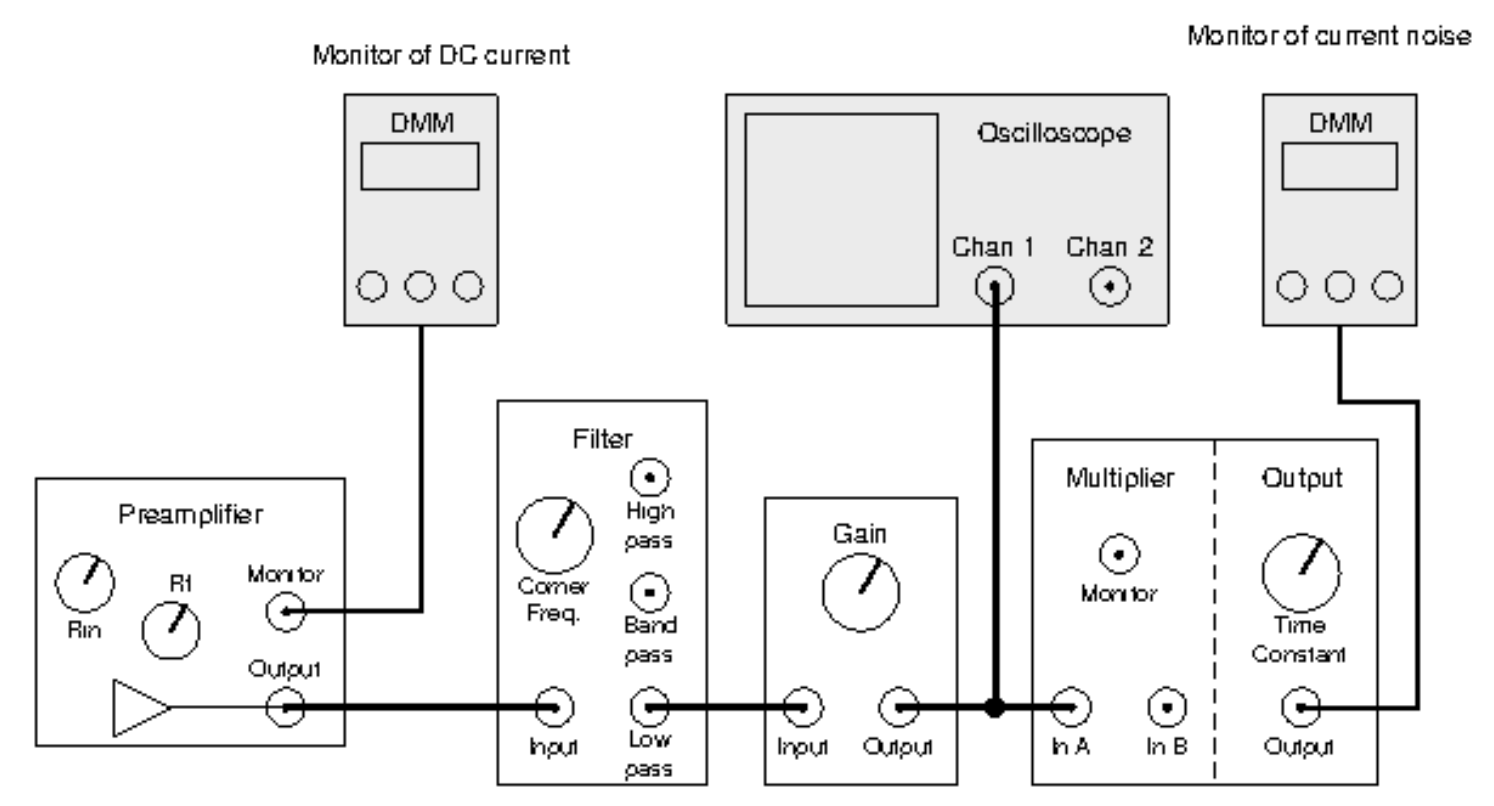
\includegraphics[width=.5\textwidth]{425_schaltplan_messung_schrot.png}
	\caption{Schaltplan zur Messung des Schrotrauschens.\cite{anleitung425}} \label{fig:schaltplan_schrot_mess}
\end{figure}

\subsection{Durchführung \& Auswertung: Messung des Schrotrauschens}
Um den linearen Bereich der Messgeräte zu verwenden, wurde der Gain für jeden Messpunkt so eingestellt, dass die Werte auf dem DMM zwischen $\SI{0.6}{V}$ und $\SI{1.2}{V}$ lagen.
Der Widerstand in der LLE--Box betrug $R_f=\SI{10}{k\ohm}$.
Da der Strom, den der OpAmp zieht, vernachlässigbar klein ist, fließt $i_\text{dc}$ vollständig durch $R_f$, wodurch
\begin{align}
	V_\text{monitor}=-R_fi_\text{dc}
	.\end{align}
Das Schrotrauschen im Schaltkreis war dann gegeben durch
\begin{align}
	\overline{\delta i^2}=\dfrac{\overline{V_\text{meter}(t)}\SI{10}{V}}{(100G_2R_f)^2}
	,\end{align}
mit $\overline{V_\text{meter}(t)}$ dem auf dem DMM abgelesenen Wert und $G_2$ dem Gain der HLE--Box.

\subsubsection{Untergrundbeiträge}
Das gemessene Rauschen entsteht nicht ausschließlich durch das Schrotrauschen.

Das \textsc{Johnson}--Rauschen im $R_f$ Widerstand liefert einen Beitrag.
Um diesen zu berechnen wurde die Ausgabe von $\overline{V_\text{meter}(t)}$ bei ausgeschalteter Lampe gemessen.
Diese liegt bei
\begin{align}
	V_\text{meter}^\text{J}=\SI{1.075+-0.005}{V}[1\%]\qquad G_2=6000
	.\end{align}
Der Operationsverstärker hat eine gewisse Offset--Spannung bei ausgeschalteter Lampe für $i_\text{dc}=\SI{0}{V}$.
Diese beträgt
\begin{align}
	V_\text{monitor}^\text{OpAmp}=\SI{-0.4+-0.1}{mV}[25\%] % TODO: Wenn wir hier die Differenz nehmen, bekommmen wir noch den Anteil von dem Bauteil dazwischen
	.\end{align}
Das Aus-- und Einstecken des DMMs ist eine mögliche Quelle für ein weiteres Rauschen, allderdings zeigte dies keinen Effekt an $V_\text{monitor}$.

Diese Beiträge werden in den folgenden Berechnungen berücksichtigt.

\subsubsection{Abhängigkeit $i_\text{dc}$}
Für unterschiedliche Spannungen der Glühlampe stellte sich ein unterschiedlich starkes Rauschen ein, da dieses linear von $i_\text{dc}$ abhängt.
Die Messwerte sind Tab. (\ref{tab:schrot_idc}) zu entnehmen. $\overline{\delta i^2}$ gegen $i_\text{dc}$ ist in Abb.\ (\ref{fig:abhängig_idc}) dargestellt.  
Die Parameter der Anpassung sind in Tab. (\ref{tab:abhängig_idc_parameter}) eingetragen.

 Da $\chi^2/\text{ddof}=\SI{1.648}{}$, sind die Messunsicherheiten sehr gut eingeschätzt worden.

Es ist $R_f=\SI{10}{k\ohm}$ und $\Delta f_\text{eff}=\SI{111051}{Hz}$.
Der lineare Zusammenhang lässt sich klar erkennen. $\Delta f_\text{eff}$ hat keine Messunsicherheit, da der eingestellte Wert $f_l=\SI{100}{\kilo Hz}$ verwendet wurde, um mit $\Delta f_{\text{eff}}=\frac{f_l\pi}{2^{3/2}}$ die effektive Bandbreite zu berechnen. %TODO chi² oder ist nur guide für auge?

Die Elementarladung bestimmt sich über den Geradenfit
\begin{align}
	e^{i_\text{dc}}=\dfrac{m}{2\Delta f_\text{eff}}
	.\end{align}
Damit
\begin{align}
	e^{i_\text{dc}} & =\SI{1.823+-0.017e-19}{C}[1\%,12.9\sigma] \\
	e^\text{lit}    & =\SI{1.602e-19}{C}
	.\end{align}
Der Literaturwert ist CODATA\cite{codataElementarladung} entnommen.
Die Abweichung von dem Literaturwert ist groß und der relative Fehler sehr klein.
Das bedeutet, dass kein statistischer Fehler sondern ein systematischer Fehler für diese große Abweichung gesorgt hat.
Auch hier gilt die selbe Begründung wie bei der Bestimmung von $k_B$.

\begin{figure}[t]
	\centering
	\resizebox{.5\textwidth}{!}{% GNUPLOT: LaTeX picture with Postscript
\begingroup
  \makeatletter
  \providecommand\color[2][]{%
    \GenericError{(gnuplot) \space\space\space\@spaces}{%
      Package color not loaded in conjunction with
      terminal option `colourtext'%
    }{See the gnuplot documentation for explanation.%
    }{Either use 'blacktext' in gnuplot or load the package
      color.sty in LaTeX.}%
    \renewcommand\color[2][]{}%
  }%
  \providecommand\includegraphics[2][]{%
    \GenericError{(gnuplot) \space\space\space\@spaces}{%
      Package graphicx or graphics not loaded%
    }{See the gnuplot documentation for explanation.%
    }{The gnuplot epslatex terminal needs graphicx.sty or graphics.sty.}%
    \renewcommand\includegraphics[2][]{}%
  }%
  \providecommand\rotatebox[2]{#2}%
  \@ifundefined{ifGPcolor}{%
    \newif\ifGPcolor
    \GPcolortrue
  }{}%
  \@ifundefined{ifGPblacktext}{%
    \newif\ifGPblacktext
    \GPblacktexttrue
  }{}%
  % define a \g@addto@macro without @ in the name:
  \let\gplgaddtomacro\g@addto@macro
  % define empty templates for all commands taking text:
  \gdef\gplbacktext{}%
  \gdef\gplfronttext{}%
  \makeatother
  \ifGPblacktext
    % no textcolor at all
    \def\colorrgb#1{}%
    \def\colorgray#1{}%
  \else
    % gray or color?
    \ifGPcolor
      \def\colorrgb#1{\color[rgb]{#1}}%
      \def\colorgray#1{\color[gray]{#1}}%
      \expandafter\def\csname LTw\endcsname{\color{white}}%
      \expandafter\def\csname LTb\endcsname{\color{black}}%
      \expandafter\def\csname LTa\endcsname{\color{black}}%
      \expandafter\def\csname LT0\endcsname{\color[rgb]{1,0,0}}%
      \expandafter\def\csname LT1\endcsname{\color[rgb]{0,1,0}}%
      \expandafter\def\csname LT2\endcsname{\color[rgb]{0,0,1}}%
      \expandafter\def\csname LT3\endcsname{\color[rgb]{1,0,1}}%
      \expandafter\def\csname LT4\endcsname{\color[rgb]{0,1,1}}%
      \expandafter\def\csname LT5\endcsname{\color[rgb]{1,1,0}}%
      \expandafter\def\csname LT6\endcsname{\color[rgb]{0,0,0}}%
      \expandafter\def\csname LT7\endcsname{\color[rgb]{1,0.3,0}}%
      \expandafter\def\csname LT8\endcsname{\color[rgb]{0.5,0.5,0.5}}%
    \else
      % gray
      \def\colorrgb#1{\color{black}}%
      \def\colorgray#1{\color[gray]{#1}}%
      \expandafter\def\csname LTw\endcsname{\color{white}}%
      \expandafter\def\csname LTb\endcsname{\color{black}}%
      \expandafter\def\csname LTa\endcsname{\color{black}}%
      \expandafter\def\csname LT0\endcsname{\color{black}}%
      \expandafter\def\csname LT1\endcsname{\color{black}}%
      \expandafter\def\csname LT2\endcsname{\color{black}}%
      \expandafter\def\csname LT3\endcsname{\color{black}}%
      \expandafter\def\csname LT4\endcsname{\color{black}}%
      \expandafter\def\csname LT5\endcsname{\color{black}}%
      \expandafter\def\csname LT6\endcsname{\color{black}}%
      \expandafter\def\csname LT7\endcsname{\color{black}}%
      \expandafter\def\csname LT8\endcsname{\color{black}}%
    \fi
  \fi
    \setlength{\unitlength}{0.0500bp}%
    \ifx\gptboxheight\undefined%
      \newlength{\gptboxheight}%
      \newlength{\gptboxwidth}%
      \newsavebox{\gptboxtext}%
    \fi%
    \setlength{\fboxrule}{0.5pt}%
    \setlength{\fboxsep}{1pt}%
    \definecolor{tbcol}{rgb}{1,1,1}%
\begin{picture}(7200.00,4320.00)%
    \gplgaddtomacro\gplbacktext{%
      \csname LTb\endcsname%%
      \put(634,619){\makebox(0,0)[r]{\strut{}$0.5$}}%
      \csname LTb\endcsname%%
      \put(634,963){\makebox(0,0)[r]{\strut{}$1$}}%
      \csname LTb\endcsname%%
      \put(634,1308){\makebox(0,0)[r]{\strut{}$1.5$}}%
      \csname LTb\endcsname%%
      \put(634,1652){\makebox(0,0)[r]{\strut{}$2$}}%
      \csname LTb\endcsname%%
      \put(634,1997){\makebox(0,0)[r]{\strut{}$2.5$}}%
      \csname LTb\endcsname%%
      \put(634,2341){\makebox(0,0)[r]{\strut{}$3$}}%
      \csname LTb\endcsname%%
      \put(634,2686){\makebox(0,0)[r]{\strut{}$3.5$}}%
      \csname LTb\endcsname%%
      \put(634,3030){\makebox(0,0)[r]{\strut{}$4$}}%
      \csname LTb\endcsname%%
      \put(634,3374){\makebox(0,0)[r]{\strut{}$4.5$}}%
      \csname LTb\endcsname%%
      \put(634,3719){\makebox(0,0)[r]{\strut{}$5$}}%
      \csname LTb\endcsname%%
      \put(731,425){\makebox(0,0){\strut{}$0$}}%
      \csname LTb\endcsname%%
      \put(1291,425){\makebox(0,0){\strut{}$10$}}%
      \csname LTb\endcsname%%
      \put(1850,425){\makebox(0,0){\strut{}$20$}}%
      \csname LTb\endcsname%%
      \put(2410,425){\makebox(0,0){\strut{}$30$}}%
      \csname LTb\endcsname%%
      \put(2969,425){\makebox(0,0){\strut{}$40$}}%
      \csname LTb\endcsname%%
      \put(3529,425){\makebox(0,0){\strut{}$50$}}%
      \csname LTb\endcsname%%
      \put(4088,425){\makebox(0,0){\strut{}$60$}}%
      \csname LTb\endcsname%%
      \put(4648,425){\makebox(0,0){\strut{}$70$}}%
      \csname LTb\endcsname%%
      \put(5207,425){\makebox(0,0){\strut{}$80$}}%
      \csname LTb\endcsname%%
      \put(5767,425){\makebox(0,0){\strut{}$90$}}%
      \csname LTb\endcsname%%
      \put(6326,425){\makebox(0,0){\strut{}$100$}}%
      \csname LTb\endcsname%%
      \put(6886,425){\makebox(0,0){\strut{}$110$}}%
    }%
    \gplgaddtomacro\gplfronttext{%
      \csname LTb\endcsname%%
      \put(6123,986){\makebox(0,0)[r]{\strut{}Daten}}%
      \csname LTb\endcsname%%
      \put(6123,793){\makebox(0,0)[r]{\strut{}Anpassung}}%
      \csname LTb\endcsname%%
      \put(170,2169){\rotatebox{-270.00}{\makebox(0,0){\strut{}$\overline{\delta i^2}/\SI{}{\nano A^2}$}}}%
      \csname LTb\endcsname%%
      \put(3809,135){\makebox(0,0){\strut{}$i_{\text{dc}}/\SI{}{\micro A}$}}%
      \csname LTb\endcsname%%
      \put(3809,4009){\makebox(0,0){\strut{}$\chi^2/\text{ddof}=\SI{1.648}{}$}}%
    }%
    \gplbacktext
    \put(0,0){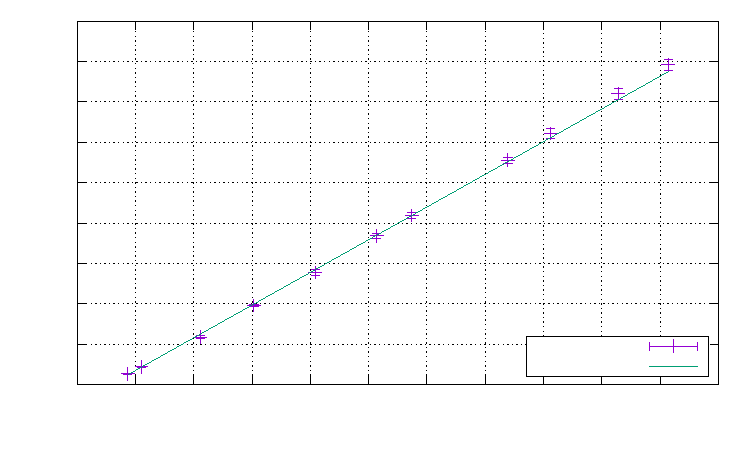
\includegraphics[width={360.00bp},height={216.00bp}]{idc}}%
    \gplfronttext
  \end{picture}%
\endgroup
}
	\caption{Stromabhängigkeit mit $\overline{\delta i^2}=\frac{V_{\text{meter}}\SI{10}{V}}{(100G_2R_f)^2}$ und $i_{\text{dc}}=-\frac{V_{\text{monitor}}}{R_f}$} \label{fig:abhängig_idc}
\end{figure}
\begin{table}[t]
	\begin{tabular}{cc}
		\toprule
		\textbf{Parameter} & {\textbf{Wert(Fehler)}}    \\
		\midrule
		m                  & \SI{4.049 \pm 0.038e-14}{A^2\per A} \\
		b                  & \SI{2.690 \pm 0.087e-19}{A^2} \\
		\bottomrule
	\end{tabular}
	\caption{Stromabhängigkeit modelliert mit $\overline{\delta i^2}(i_{\text{dc}})=m\cdot i_{\text{dc}}+b$} \label{tab:abhängig_idc_parameter}
\end{table}

\subsubsection{Abhängigkeit $\Delta f_\text{eff}$}
Für $i_\text{dc}=\text{const.}$ wurde durch Variation der Bandbreite die Weißheit des Rauschens überprüft.
Die Weißheit gibt an, wie sich das Rauschen bei unterschiedlichen Frequenzen verhält.
Es ist weiß, wenn es frequenzunabhängig ist.
$\overline{\Delta i^2}$ ist gegen $\Delta f_{\text{eff}}$ in Abb.\ (\ref{fig:abhängig_f}) aufgetragen. Die Messwerte sind Tab. (\ref{tab:schrot_freq}) zu entnehmen.
Die Parameter für den Fit sind in Tab.\ (\ref{tab:abhängig_f_parameter}) eingetragen. %TODO chi² oder auch nur guide?

Da $\chi^2/\text{ddof}=\SI{2.017}{}$, sind die Messunsicherheiten ebenfalls repräsentativ.

Wie erwartet ist zu erkennen, dass der Rauschstrom linear mit der Bandbreite steigt.
Das bedeutet, dass das für die Vergrößerung der Bandbreite immer eine konstante Rauschspannung addiert wird.
Das Rauschen ist also nur abhängig von der Bandbreite und unabhängig von der Frequenz selbst.
Dieses Verhalten war zu erwarten, weil das Schrotrauschen weißes Rauschen ist.

Die Elementarladung bestimmt sich über den Geradenfit
\begin{align}
	e^{\Delta f_\text{eff}}=\dfrac{m}{2i_\text{dc}}
	.\end{align}
Damit
\begin{align}
	e^{\Delta f_\text{eff}} & =\SI{1.958+-0.039e-19}{C}[2\%,10\sigma] \\
	e^\text{lit}            & =\SI{1.602e-19}{C}
\end{align}
Der Literaturwert ist CODATA\cite{codataElementarladung} entnommen.
Die Abweichung von dem Literaturwert ist auch für dieses Verfahren groß und die relative Fehler klein.
Dieser Wert unterscheidet sich nicht stark von $e^{i_\text{dc}}$; da der relative Fehler größer ist, ist die Abweichung kleiner.
Hier gilt die selbe Diskussion.

\begin{figure}[t]
	\centering
	\resizebox{.5\textwidth}{!}{% GNUPLOT: LaTeX picture with Postscript
\begingroup
  \makeatletter
  \providecommand\color[2][]{%
    \GenericError{(gnuplot) \space\space\space\@spaces}{%
      Package color not loaded in conjunction with
      terminal option `colourtext'%
    }{See the gnuplot documentation for explanation.%
    }{Either use 'blacktext' in gnuplot or load the package
      color.sty in LaTeX.}%
    \renewcommand\color[2][]{}%
  }%
  \providecommand\includegraphics[2][]{%
    \GenericError{(gnuplot) \space\space\space\@spaces}{%
      Package graphicx or graphics not loaded%
    }{See the gnuplot documentation for explanation.%
    }{The gnuplot epslatex terminal needs graphicx.sty or graphics.sty.}%
    \renewcommand\includegraphics[2][]{}%
  }%
  \providecommand\rotatebox[2]{#2}%
  \@ifundefined{ifGPcolor}{%
    \newif\ifGPcolor
    \GPcolortrue
  }{}%
  \@ifundefined{ifGPblacktext}{%
    \newif\ifGPblacktext
    \GPblacktexttrue
  }{}%
  % define a \g@addto@macro without @ in the name:
  \let\gplgaddtomacro\g@addto@macro
  % define empty templates for all commands taking text:
  \gdef\gplbacktext{}%
  \gdef\gplfronttext{}%
  \makeatother
  \ifGPblacktext
    % no textcolor at all
    \def\colorrgb#1{}%
    \def\colorgray#1{}%
  \else
    % gray or color?
    \ifGPcolor
      \def\colorrgb#1{\color[rgb]{#1}}%
      \def\colorgray#1{\color[gray]{#1}}%
      \expandafter\def\csname LTw\endcsname{\color{white}}%
      \expandafter\def\csname LTb\endcsname{\color{black}}%
      \expandafter\def\csname LTa\endcsname{\color{black}}%
      \expandafter\def\csname LT0\endcsname{\color[rgb]{1,0,0}}%
      \expandafter\def\csname LT1\endcsname{\color[rgb]{0,1,0}}%
      \expandafter\def\csname LT2\endcsname{\color[rgb]{0,0,1}}%
      \expandafter\def\csname LT3\endcsname{\color[rgb]{1,0,1}}%
      \expandafter\def\csname LT4\endcsname{\color[rgb]{0,1,1}}%
      \expandafter\def\csname LT5\endcsname{\color[rgb]{1,1,0}}%
      \expandafter\def\csname LT6\endcsname{\color[rgb]{0,0,0}}%
      \expandafter\def\csname LT7\endcsname{\color[rgb]{1,0.3,0}}%
      \expandafter\def\csname LT8\endcsname{\color[rgb]{0.5,0.5,0.5}}%
    \else
      % gray
      \def\colorrgb#1{\color{black}}%
      \def\colorgray#1{\color[gray]{#1}}%
      \expandafter\def\csname LTw\endcsname{\color{white}}%
      \expandafter\def\csname LTb\endcsname{\color{black}}%
      \expandafter\def\csname LTa\endcsname{\color{black}}%
      \expandafter\def\csname LT0\endcsname{\color{black}}%
      \expandafter\def\csname LT1\endcsname{\color{black}}%
      \expandafter\def\csname LT2\endcsname{\color{black}}%
      \expandafter\def\csname LT3\endcsname{\color{black}}%
      \expandafter\def\csname LT4\endcsname{\color{black}}%
      \expandafter\def\csname LT5\endcsname{\color{black}}%
      \expandafter\def\csname LT6\endcsname{\color{black}}%
      \expandafter\def\csname LT7\endcsname{\color{black}}%
      \expandafter\def\csname LT8\endcsname{\color{black}}%
    \fi
  \fi
    \setlength{\unitlength}{0.0500bp}%
    \ifx\gptboxheight\undefined%
      \newlength{\gptboxheight}%
      \newlength{\gptboxwidth}%
      \newsavebox{\gptboxtext}%
    \fi%
    \setlength{\fboxrule}{0.5pt}%
    \setlength{\fboxsep}{1pt}%
    \definecolor{tbcol}{rgb}{1,1,1}%
\begin{picture}(7200.00,4320.00)%
    \gplgaddtomacro\gplbacktext{%
      \csname LTb\endcsname%%
      \put(829,619){\makebox(0,0)[r]{\strut{}$0.001$}}%
      \csname LTb\endcsname%%
      \put(829,1491){\makebox(0,0)[r]{\strut{}$0.01$}}%
      \csname LTb\endcsname%%
      \put(829,2362){\makebox(0,0)[r]{\strut{}$0.1$}}%
      \csname LTb\endcsname%%
      \put(829,3234){\makebox(0,0)[r]{\strut{}$1$}}%
      \csname LTb\endcsname%%
      \put(829,4106){\makebox(0,0)[r]{\strut{}$10$}}%
      \csname LTb\endcsname%%
      \put(927,425){\makebox(0,0){\strut{}$0.1$}}%
      \csname LTb\endcsname%%
      \put(2417,425){\makebox(0,0){\strut{}$1$}}%
      \csname LTb\endcsname%%
      \put(3907,425){\makebox(0,0){\strut{}$10$}}%
      \csname LTb\endcsname%%
      \put(5396,425){\makebox(0,0){\strut{}$100$}}%
      \csname LTb\endcsname%%
      \put(6886,425){\makebox(0,0){\strut{}$1000$}}%
    }%
    \gplgaddtomacro\gplfronttext{%
      \csname LTb\endcsname%%
      \put(170,2362){\rotatebox{-270}{\makebox(0,0){\strut{}$\overline{\delta i^2}/\SI{}{\nano V^2}$}}}%
      \csname LTb\endcsname%%
      \put(3906,135){\makebox(0,0){\strut{}$\Delta f_{\text{eff}}/\SI{}{\kilo Hz}$}}%
      \csname LTb\endcsname%%
      \put(6123,986){\makebox(0,0)[r]{\strut{}Daten}}%
      \csname LTb\endcsname%%
      \put(6123,793){\makebox(0,0)[r]{\strut{}Anpassung}}%
    }%
    \gplbacktext
    \put(0,0){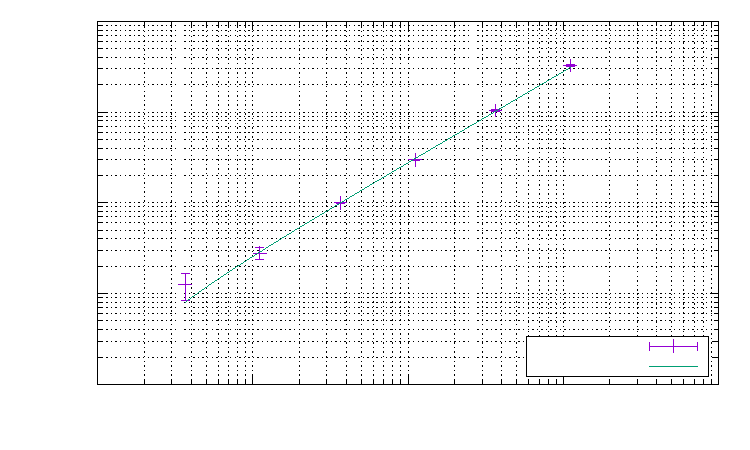
\includegraphics[width={360.00bp},height={216.00bp}]{shot_freq}}%
    \gplfronttext
  \end{picture}%
\endgroup
}
	\caption{Frequenzabhängigkeit mit $\overline{\delta i^2}=\frac{V_{\text{meter}}\SI{10}{V}}{(100G_2R_f)^2}$ und $\Delta f_{\text{eff}}=\frac{f_l\pi}{2^{3/2}}$} \label{fig:abhängig_f}
\end{figure}
\begin{table}[t]
	\begin{tabular}{cc}
		\toprule
		\textbf{Parameter} & {\textbf{Wert(Fehler)}}    \\
		\midrule
		m                  & \SI{2.784 \pm 0.056e-23}{A^2\per Hz} \\
		b                  & \SI{-2.2 \pm 3.0e-21}{A^2}    \\
		\bottomrule
	\end{tabular}
	\caption{Frequenzabhängigkeit modelliert mit $\overline{\delta i^2}(f)=m\cdot f+b$} \label{tab:abhängig_f_parameter}
\end{table}

\iffalse\subsubsection{Vergleich $i_\text{dc}$ und $\Delta f_\text{eff}$}
Vergleicht man die berechneten Elementarladungen so liegt die Abweichung bei
\begin{align}
	e^{i_\text{dc}}                           & =\SI{1.823+-0.017e-19}{C}[1\%,12.9\sigma ] \\
	e^{\Delta f_\text{eff}}                   & =\SI{1.958+-0.039e-19}{C}[2\%,9.1\sigma ]  \\
	|e^{i_\text{dc}}-e^{\Delta f_\text{eff}}| & =\SI{0.135+-0.043e-19}{C}
	.\end{align}
\fi

\section{Fazit}
Ein Bandpass liefert eine Bandbreite von
\begin{align}
	\Delta f_\text{eff}=\int_{0}^{\infty}\td fG_\text{HP}^2(f)G_\text{LP}^2(f)=\dfrac{f_\text{l}^4\pi \left(f_\text{h}-f_\text{l}\right)}{2^{3/2}\left(f_\text{h}^4-f_\text{l}^4\right)}
	.\end{align}
Dieser Formel stimmt gut mit der gemessenen Bandbreite überein und konnte für diesen Versuch verwendet werden.

Das \textsc{Johnson}--Rauschen, oder thermisches Rauschen, beschreibt das Rauschen in einem Widerstand $R$ bei Temperatur $T$ für eine gewisse Bandbreite $\Delta f_\text{eff}$
\begin{align}
	\overline{V_\text{J}^2}=4k_BTR\Delta _\text{eff}
	.\end{align}
Hieraus lässt sich, mit Variation des Widerstands oder der Bandbreite, die \textsc{Boltzmann}--Konstante bestimmen, zu
\begin{align}
	k_B^R & = \SI{11.53+-0.09e-23}{J/K}[1\%,112.7\sigma ] \\
	k_B^f & = \SI{6.756+-0.06e-23}{J/K}[1\%,89.6\sigma ]
	.\end{align}
Die Abweichung von der Literatur sind bei sehr kleinem relativem Fehler sehr groß, was auf systematische Fehler hinweist, wie die Änderung der gemessenen Spannung bei einer Geräuschkulisse(!).

Das Schrotrauschen entsteht durch die Quantelung der Elementarladung in $e$.
Wenn Ladungsträger eine Potentialbarriere überwinden, dann ist die transferierte Ladung nicht kontinuierlich, was zu Strom-- und Spannungsimpulsen führt.
Das Rauschen hängt also von der Ladung $e$, dem angelegten Gleichstrom $i_\text{dc}$ und der Bandbreite $\Delta f_\text{eff}$ ab, wie
\begin{align}
	\overline{\delta i^2}=2ei_\text{dc}\Delta f_\text{eff}
	.\end{align}
Da hier nur ein Tiefpass verwendet worden ist, ist $\Delta f_\text{eff}=\tfrac{f_\text{l}\pi }{2^{3/2}}$.
Die Elementarladung kann dann über Variation von $i_\text{dc}$ oder $\Delta f_\text{eff}$ berechnet werden, zu
\begin{align}
	e^{i_\text{dc}}         & = \SI{1.823+-0.017e-19}{C}[1\%,12.9\sigma ] \\
	e^{\Delta f_\text{eff}} & = \SI{1.958+-0.039e-19}{C}[2\%,10\sigma ]
	.\end{align}
Die Abweichung von der Literatur ist zwar signifikant kleiner als bei der \textsc{Boltzmann}--Konstante, allerdings nicht im erwarteten Intervall.
Da hier auch die statistischen Fehler sehr gering sind, muss es sich hier um die selben systematischen Fehler, wie bei der \textsc{Boltzmann}--Konstante handeln.

Beide Rauschtypen sind weißes Rauschen, was mit einem linearen Zusammenhang zwischen der Rauschspannung und der Bandbreite gezeigt wurde.

\clearpage
\section{Appendix}
\begin{table}[h]
	\begin{tabular}{S[table-format=1.2e1] S[table-format=1.2] S[table-format=1.2] S[table-format=1.2e1] S[table-format=1.2e1]}
		\toprule
		{\(f\,[\si{\hertz}]\)} & {\(U_0\,[\si{\volt}]\)} & {\(\Delta U_0\,[\si{\volt}]\)} & {\(U\,[\si{\volt}]\)} & {\(\Delta U\,[\si{\volt}]\)} \\
		\midrule
		2                      & 5.95                    & 0.01                           & 6e-3                  & 10e-3                        \\
		8                      & 7.35                    & 0.01                           & 45e-3                 & 10e-3                        \\
		2e1                    & 7.40                    & 0.01                           & 295e-3                & 10e-3                        \\
		8e1                    & 7.50                    & 0.01                           & 4.01                  & 0.05                         \\
		2e2                    & 7.50                    & 0.01                           & 7.27                  & 0.05                         \\
		8e2                    & 7.50                    & 0.05                           & 7.51                  & 0.05                         \\
		2e3                    & 7.50                    & 0.05                           & 7.51                  & 0.05                         \\
		8e3                    & 7.47                    & 0.05                           & 6.33                  & 0.05                         \\
		2e4                    & 7.44                    & 0.05                           & 1.83                  & 0.05                         \\
		8e4                    & 7.45                    & 0.05                           & 119e-3                & 5e-3                         \\
		2e5                    & 7.45                    & 0.05                           & 20e-3                 & 2e-3                         \\
		8e5                    & 7.45                    & 0.05                           & 1.5e-3                & 1e-3                         \\
		2e6                    & 7.40                    & 0.04                           & 1e-3                  & 1e-3                         \\
		8e6                    & 7.70                    & 0.10                           & 1e-3                  & 1e-3                         \\
		\bottomrule
	\end{tabular}
	\caption{Messdaten zur Vermessung der Bandbreite (\ref{sec:bandbreite}).}
	\label{tab:frequency_data}
\end{table}

\begin{table}[h]
	\begin{tabular}{S[table-format=3.1e1] S[table-format=3e1] S[table-format=1e1] S[table-format=1.2] S[table-format=2e1]}
		\toprule
		$f_\text{l}[\SI{}{Hz}]$ & $f_\text{h}[\SI{}{Hz}]$ & $G_{2}$ & $V_\text{meter}\left[\SI{}{V}\right]$ & $\Delta V_\text{meter}\left[\SI{}{V}\right]$ \\
		\midrule
		3.3e3                   & 1e1                     & 1e4     & 1.05                                  & 10e-3                                        \\
		3.3e3                   & 1e2                     & 1e4     & 1.01                                  & 1e-2                                         \\
		3.3e3                   & 3e2                     & 1e4     & 0.95                                  & 1e-2                                         \\
		3.3e3                   & 1e3                     & 1e4     & 0.73                                  & 1e-2                                         \\
		10e3                    & 1e3                     & 6e3     & 1.01                                  & 1e-2                                         \\
		10e3                    & 4e3                     & 6e3     & 0.79                                  & 1e-2                                         \\
		33e3                    & 100                     & 3e3     & 0.93                                  & 1e-2                                         \\
		33e3                    & 300                     & 3e3     & 0.92                                  & 1e-2                                         \\
		33e3                    & 1e3                     & 3e3     & 0.91                                  & 1e-2                                         \\
		33e3                    & 3e3                     & 3e3     & 0.86                                  & 1e-2                                         \\
		100e3                   & 100                     & 2e3     & 1.27                                  & 1e-2                                         \\
		100e3                   & 300                     & 2e3     & 1.26                                  & 1e-2                                         \\
		100e3                   & 1e3                     & 2e3     & 1.26                                  & 1e-2                                         \\
		100e3                   & 3e3                     & 2e3     & 1.24                                  & 1e-2                                         \\
		\bottomrule
	\end{tabular}
	\caption{Messdaten zur Vermessung des \textsc{Johnson}--Rauschens mit der Variation der Bandbreite.}
	\label{tab:john_freq}
\end{table}

\begin{table}[h]
	\begin{tabular}{S[table-format=1e1]S[table-format=1.1e1]S[table-format=1.3]S[table-format=2e1]}
		\toprule
		$R_\text{in}[\SI{}{\ohm}]$ & $G_{2}$ & $V_\text{meter}[\SI{}{V}]$ & $\Delta V_\text{meter}[\SI{}{V}]$ \\
		\midrule
		1e0                        & 2e3     & 1                          & 12e-3                             \\
		1e1                        & 2e3     & 1.002                      & 12e-3                             \\
		1e2                        & 2e3     & 1.027                      & 12e-3                             \\
		1e3                        & 1.5e3   & 0.714                      & 13e-3                             \\
		1e4                        & 1e3     & 0.920                      & 12e-3                             \\
		1e5                        & 4e2     & 0.828                      & 12e-3                             \\
		1e6                        & 3e2     & 0.856                      & 14e-3                             \\
		\bottomrule
	\end{tabular}
	\caption{Messdaten zur Vermessung des \textsc{Johnson}--Rauschens mit der Variation des Widerstands.}
	\label{tab:john_wid}
\end{table}

\begin{table}[h]
	\begin{tabular}{S[table-format=1.1e1]S[table-format=1.1e2]S[table-format=1.3]S[table-format=1.3]}
		\toprule
		$f_\text{l}[\SI{}{Hz}]$ & $G_{2}$ & $V_\text{meter}[\SI{}{V}]$ & $\Delta V_\text{meter}[\SI{}{Hz}]$ \\
		\midrule
		330                     & 10e3    & 0.125                      & 0.040                              \\
		1e3                     & 10e3    & 0.28                       & 0.04                               \\
		3.3e3                   & 10e3    & 1.0                        & 0.02                               \\
		10e3                    & 6e3     & 1.07                       & 0.02                               \\
		33e3                    & 3e3     & 0.93                       & 0.02                               \\
		100e3                   & 1.5e3   & 0.731                      & 0.02                               \\
		\bottomrule
	\end{tabular}
	\caption{Messdaten zur Vermessung des Schrotrauschens in Abhängigkeit von $\Delta f_\text{eff}$.}
	\label{tab:schrot_freq}
\end{table}

\begin{table}[h]
	\begin{tabular}{S[table-format=-3.1e1]S[table-format=1.1e1]S[table-format=1.3]S[table-format=1.3]}
		\toprule
		$i_\text{dc}[\SI{}{V}]$ & $G_{2}$ & $I[\SI{}{A}]$ & $\Delta I[\SI{}{V}]$ \\
		\midrule
		-86.9e-3                & 4e3     & 1.008         & 0.012                \\
		-109.8e-3               & 4e3     & 1.147         & 0.012                \\
		-211.5e-3               & 3e3     & 0.977         & 0.014                \\
		-303.2e-3               & 3e3     & 1.328         & 0.014                \\
		-408e-3                 & 2e3     & 0.755         & 0.015                \\
		-514e-3                 & 2e3     & 0.936         & 0.014                \\
		-574e-3                 & 2e3     & 1.036         & 0.015                \\
		-739e-3                 & 2e3     & 1.312         & 0.015                \\
		-812e-3                 & 1.5e3   & 0.812         & 0.015                \\
		-928e-3                 & 1.5e3   & 0.923         & 0.015                \\
		-1014e-3                & 1.5e3   & 1.004         & 0.015                \\
		\bottomrule
	\end{tabular}
	\caption{Messdaten zur Vermessung des Schrotrauschens in Abhängigkeit von $i_\text{dc}$.}
	\label{tab:schrot_idc}
\end{table}

\bibliography{refs}

\end{document}
